\documentclass{article}
\usepackage{tikz}
\usetikzlibrary{datavisualization.formats.functions}
\newcommand{\probe}[2]{\pgfextractx{\dimen0}{\pgfpointanchor{#1}{#2}}\pgfextracty{\dimen2}{\pgfpointanchor{#1}{#2}}\typeout{POINT #1.#2: \the\dimen0,\the\dimen2}}
\begin{document}
\pgfmathsetseed{100}
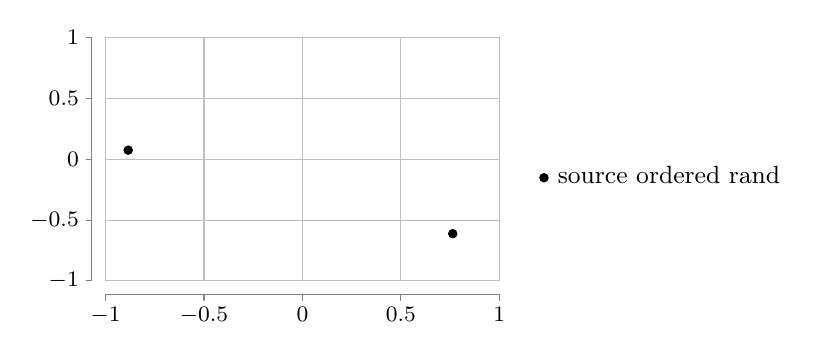
\begin{tikzpicture}
\datavisualization [scientific axes=clean,
  x axis={min value=-1,max value=1,ticks={step=.5},grid},
  y axis={min value=-1,max value=1,ticks={step=.5},grid},
  visualize as scatter,
  legend={matrix node style={name=legend},label style={node style={name=label}}},
  scatter={style={mark=*,mark size=1.5pt},label in legend={text={source ordered rand}}}]
data [format=function] {
  var i : interval [0:1] samples 2;
  func y = rand;
  func x = rand;
};
\probe{data visualization bounding box}{south west}
\probe{data visualization bounding box}{north east}
\probe{data bounding box}{south west}
\probe{data bounding box}{north east}
\probe{legend}{south west}\probe{legend}{north east}
\probe{label}{base west}\probe{label}{mid west}\probe{label}{center}
\end{tikzpicture}
\end{document}
